\documentclass[Kravspecifikation/Kravspec_Main.tex]{subfiles}

\begin{document}
\section{Ordliste}
\begin{longtable}{|L{0.30\textwidth}|L{0.70\textwidth}|}
        \hline
        \textbf{Term} & \textbf{Beskrivelse} \\ \hline
        Bilprofil & Profil for udlejningsbil. Indeholder information omkring bilen, specifikt udlejningsintervaller og biludstyr. En bilprofil er oprettet og håndteres af systemet, samt tilgængelig til potentielle lejere. \\ \hline
        Brugerinfo & Gemt info om brugeren. E-mail, telefonnummer og navn \\ \hline 
        Biludstyr & Kvaliteter for en bil: Antal sæder, m/u aircondition, GPS, børnesæder. \\ \hline
        Søgningskriterier & Bilmodel, Tidsinterval for udlejning, pris og biludstyr \\ \hline 
        Bilprofil skabelon & Bilmodel, Nummerplade, Antal kilomenter og pris for bil per dag. Navn, mobilnummer, adresse, afhentningsadresse og by for biludlejer. \\ \hline 
        Hovedmenu & Den første menu brugere kommer til efter at have logget ind. Herfra kan der navigeres til alle andre menuer.\\
        \hline
        \caption{Ordliste med vigtige begreber}
        \label{tab:ordliste}
\end{longtable}
\newpage

\section{Introduktion}
I det følgende specificeres kravene for CarnGo. Dette indebærer en beskrivelse af aktørerne i systemet og af de funktionelle samt ikke-funktionelle krav. For at beskrive hvad der interagerer med eller påvirker systemet, er der lavet et aktør-kontekst diagram med tilhørende aktør beskrivelser. Systemets funktionalitet og brugsscenarier beskrives med udgangspunkt i user stories. Dette er en mere agil tilgang til krav, og user stories afviger fra klassiske krav ved at være uformelle beskrivelser af systemets features. Der tages udgangspunkt i brugeren, og formålet er, at skabe en fælles forståelse for systemet og dets kontekst. For at bidrage til den fælles forståelse kombineres user stories med en beskrivelse af personas. De ikke-funktionelle krav er beskrevet og kategoriseret ved brug af FURPS-modellen. Desuden anvendes MoSCoW til at prioritere kravene og fastlægge vigtigheden af de enkelte krav. For definitioner af vigtige begreber henvises til ordlisten i tabel \ref{tab:ordliste}.

\section{Aktør beskrivelse}
Før systemets brug og features beskrives, bør det afklares, hvilke aktører, som anvender og interagerer med CarnGo. Dette fremgår af aktør-kontekst diagrammet i figur \ref{fig:actor_context}
\begin{figure}[H]
    \centering
    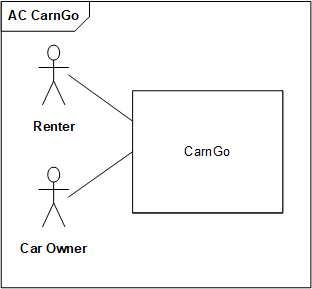
\includegraphics[width=0.5\textwidth]{Kravspecifikation/Funktionelle_krav/ActorContext/graphics/AC_CarnGo.png}
    \caption{Aktør-kontekst diagram for CarnGo}
    \label{fig:actor_context}
\end{figure}
De enkelte aktører og deres indvirkning på systemet er uddybet i tabellerne \ref{tab:RenterBeskrivelse} og \ref{tab:CarOwnerBeskrivelse} nedenfor. Andre potentielle aktører kunne være en database eller en bil. Databasen betragtes dog som en del af systemet, og ikke som en selvstændig aktør. Desuden vurderes det, at bilen er repræsenteret gennem udlejer. Den interagerer ikke selv med applikationen, men bliver udbudt af udlejer, hvorefter systemet refererer til den i en bilprofil.

\subsection{Renter}
\begin{table}[H]
    \centering
    \begin{tabular}{|L{0.35\textwidth}|L{0.65\textwidth}|}
        \hline
        \textbf{Aktør navn} & Renter \\ \hline
        \textbf{Alternativ referencer} & Lejer \\ \hline
        \textbf{Type} & Primær \\ \hline
        \textbf{Beskrivelse} & En bruger der har oprettet en lejer profil. Dette indebærer at brugeren er registreret i systemet som lejer, hvilket giver brugeren mulighed for at leje biler. \\ \hline
    \end{tabular}
    \caption{Aktør beskrivelse for Renter}
    \label{tab:RenterBeskrivelse}
\end{table}

\subsection{Car Owner}
\begin{table}[H]
    \centering
    \begin{tabular}{|L{0.35\textwidth}|L{0.65\textwidth}|}
        \hline
        \textbf{Aktør navn} & Car Owner \\ \hline
        \textbf{Alternativ referencer} & Udlejer \\ \hline
        \textbf{Type} & Primær \\ \hline
        \textbf{Beskrivelse} & En bruger der har oprettet en udlejer profil. Dette indebærer at brugeren er registreret i systemet som udlejer, hvilket giver brugeren mulighed for at oprette bilprofiler. \\ \hline
    \end{tabular}
    \caption{Aktør beskrivelse for Car OWner}
    \label{tab:CarOwnerBeskrivelse}
\end{table}

\end{document}